\documentclass{beamer}
\usepackage{ctex}
\mode<presentation>
{
  \usetheme{Madrid}      % or try Darmstadt, Madrid, Warsaw, ...
  \usecolortheme{default} % or try albatross, beaver, crane, ...
  \usefonttheme{default}  % or try serif, structurebold, ...
  \setbeamertemplate{navigation symbols}{}
  \setbeamertemplate{caption}[numbered]
} 

\usepackage[english]{babel}
\usepackage[utf8]{inputenc}
\usepackage[T1]{fontenc}

\title[Social dilemmas among unequals]{Social dilemmas among unequals}
\author{修格致}
\institute{PKU}
\date{\today}

\begin{document}

\begin{frame}
  \titlepage
\end{frame}

\begin{frame}{Outline}
 \tableofcontents
\end{frame}

\section{Introduction}

\begin{frame}{Introduction}
如何对不平等的直接互惠行为进行建模?
\begin{itemize}
  \item Your introduction goes here!
  \item Use \texttt{itemize} to organize your main points.
\end{itemize}
如何验证?
\begin{itemize}
    \item equilibrium calculations, 
    \item evolutionary simulations
    \item behavioural experiment
\end{itemize}

\vskip 1cm

\begin{block}{Examples}
Some examples of commonly used commands and features are included, to help you get started.
\end{block}

\end{frame}

\section{Paper Review}

\subsection{Social dilemmas among unequals}

\begin{frame}{Social dilemmas among unequals}

\begin{itemize}
    \item Hauser, O.P., Hilbe, C., Chatterjee, K. et al. Social dilemmas among unequals. Nature 572, 524–527 (2019). https://doi.org/10.1038/s41586-019-1488-5
\end{itemize}

\end{frame}
%%%% Basics
\subsection{Basics}
\begin{frame}{几个概念\&有趣结论}
概念
\begin{itemize}
    \item \textbf{Payoff:}选择一个策略得到的回报。
    \item \textbf{直接互惠:}一种产生合作的机制。我给你挠挠背,你就给我挠挠背。条件是再次碰面的概率高于无私行为的成本收益比。
    \item \textbf{平等:}每个人相同行为的社会后果相同。
    \begin{itemize}
        \item 可以异质性的点:收入、生产能力、依赖公共资产的程度。
    \end{itemize}
    \item \textbf{合作:}人的一种行为,与对抗相对。我们希望我们的社会价值观(Payoff矩阵)可以支持我们的合作行为。
    \item \textbf{公平、效率、公益:}他们的确定决定了社会价值观。
    \end{itemize}
\only<2>{结论
\begin{itemize}
    \item 极端不平等阻碍合作。
    \item 生产能力有差异时,收入的不同可以使更多的人选择合作。
    \item 多劳多得使得社会总福利最大。多劳不多得使得社会合作迅速消失。
\end{itemize}
}
    
\end{frame}
\begin{frame}{一些矛盾点}
Social dilemmas
\begin{itemize}
    \item 每个人都选择合作时社会最大化福利。但是其他人都选择合作,背叛才收益最大化。
\end{itemize}

什么样的社会促进合作?为什么?

\begin{itemize}
    \item 稳定、长期有效的社会(名声是有用的)
\end{itemize}

已有工作怎么做?

\begin{itemize}
    \item 同质性、公平社会
\end{itemize}

问题?
\only<2>{\begin{center}
    真实世界是不同质的;同质社会难免TOC。
\end{center}}
    
\end{frame}
%%%% 模型表述
\subsection{模型表述}
\begin{frame}{框架:不公平条件下的社会困境}
变量:收入(平等)、能力(对称性)、公益/养老保险/Payoff(线性性)\\

\vspace{0.5cm}
\begin{itemize}
    \item<1-> 框架描述:\begin{itemize}
    \item $n$ players
    \item 每一轮选手$i$得到“工资”/“气力”$e_i$
    \item 得到工资后,每个人独立将某比例$x_i$的工资投入社会生产,于是公共财富的总和是$\sum_{j = 1}^n r_j e_j x_j$, 其中$r_j$是每个人的生产能力。
    \item payoff决定于$e_i$和$x_i$
\end{itemize}
\pause
\only<2>{\item 通常假设(公平社会):
\begin{itemize}
    \item $e_i$ i.i.d.
    \item 对公共物的贡献要乘一个生产率因子$r
.$
\end{itemize}}
\only<3>{\item 本文假设(不公平社会)
\begin{itemize}
    \item $e_i$各有不同
    \item $r_i$各有不同
\end{itemize}}
\end{itemize}
\end{frame}

\begin{frame}{社会困境例子:公共资源平分}
\begin{block}{收益:}
    $${u}_{i}=\frac{1}{n}\mathop{\sum }\limits_{j=1}^{n}{r}_{j}{e}_{j}{x}_{j}+(1-{x}_{i}){e}_{i}$$
这是一个社会困境:选手$i$可以通过使得 $x_i=0$ 来获益(free-ride)。
\end{block}

\begin{itemize}
    \item 要求:$r_j\in (1,n)$. (为什么?)
\end{itemize}

\vspace{0.5cm}

\only<2,3,4>{\textbf{只玩一轮:}唯一的均衡是背叛(defection);}
\vspace{0.5cm}

\only<3,4>{\textbf{进行多轮:}合作可以在player采纳一些\textit{条件策略}的时候出现,比如以眼还眼(tit-for-tat)、优胜劣汰(win-stay lose-shift)等。}
\only<4>{\begin{center}
    \textbf{假设每一轮博弈之后,有新一轮的概率为$\delta$.}
\end{center}}
\end{frame}

\begin{frame}{不公平条件下的社会困境}
    \begin{figure}
        \centering
        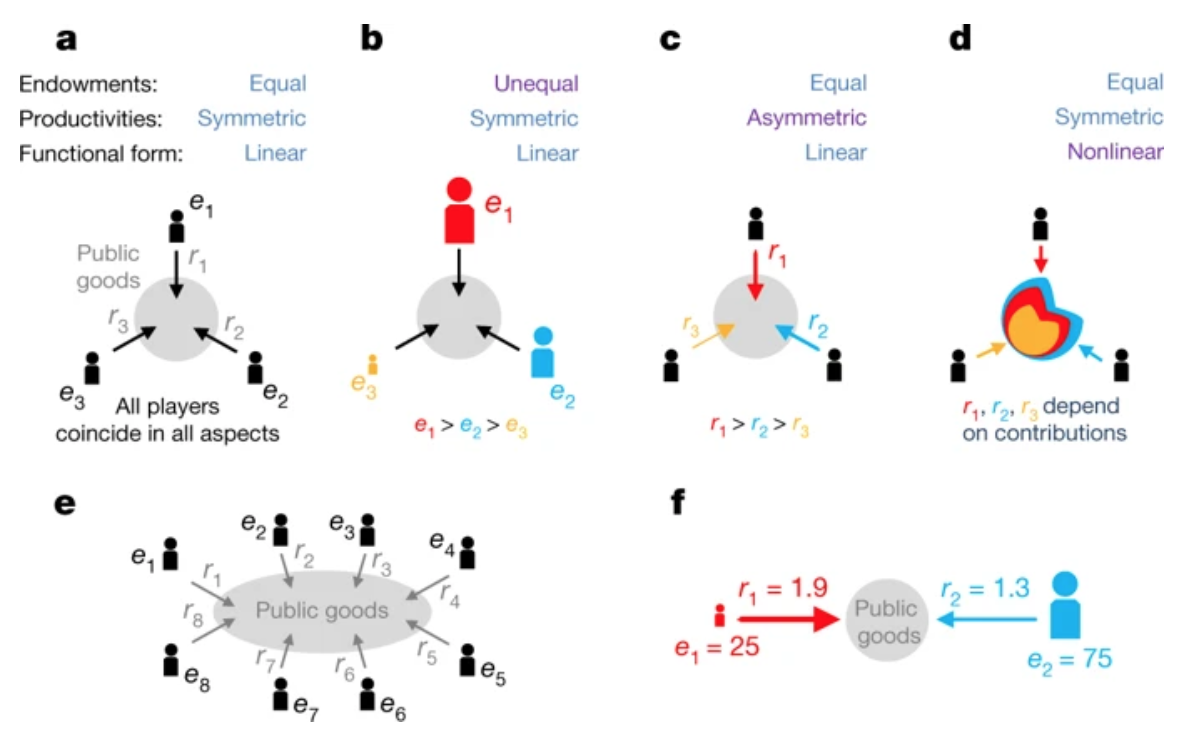
\includegraphics[width = 0.8\linewidth]{figs/sketch}
        \caption{\textbf{Public goods games among unequals.} Game Concepts: \textit{symmetric:} indistinguishable except for $e_i$, $x_i$; \textit{linear:} $r_i\equiv c$ }
        \label{fig:sketch}
    \end{figure}
\end{frame}


\begin{frame}{如何实现合作社会(feasibility)}
    如果存在完美子博弈均衡,完全合作就能出现。这种子博弈均衡指的是所有玩家都贡献出所有的财富。
    
    Grim策略:如果没人在上一轮背叛,下一轮的策略就不变,依然是全部奉献 $x_i(t) = 1$ if $\forall j,x_j(t-1) = 1$ 。该策略在如下条件满足的时候就是一个均衡:\[\frac{\delta}{n}\sum_{j\ne i}r_je_j\geq (1-\frac{r_i}{n})e_i \]
    
    即未来合作的收益必须大于本轮背叛的刺激。
\end{frame}
\subsection{一些例子与分析}
\begin{frame}{如何实现合作社会(feasibility)}
    \begin{itemize}
        \item 如果不平等太多,永远不可能达成合作。
        \item 线性、对称博弈:合作完全可以达到。
        \item 非对称、非线性博弈:完全合作只有非均等收入的时候可能出现。此时,最好每个人都没有初始收入。
    \end{itemize}
\end{frame}

\begin{frame}{Intuition:多劳多得的好处?}
如果每个人的生产能力$r_i$随$i$递减:
\begin{itemize}
    \item \textbf{稳定性:}多劳多得更容易让全体合作达到均衡。否则,$\forall i, e_i\equiv c$,则合作的适定条件:$$\delta>\frac{n-r_n}{\sum r_i -r_n} = 1 - \frac{\sum r_i -n}{\sum r_i -r_n} $$ 能力越差越可能背叛,ta的边际贡献$1-r_n/n$也最高。

\only<2,3>{
        \item \textbf{效率:}更多的工资给能力强的人,他们交税更多,使得社会资源更丰富。}
\end{itemize}
\only<3>{
\begin{center}
    多劳多得有利于社会合作适定性。
\end{center}}
\end{frame}
\begin{frame}{二人博弈的特例}
能力不同时,工资的最优均衡。
    \[\frac{{e}_{1}}{{e}_{2}}=\sqrt{\frac{{r}_{2}(2-{r}_{2})}{{r}_{1}(2-{r}_{1})}}\]
    \begin{figure}
        \centering
        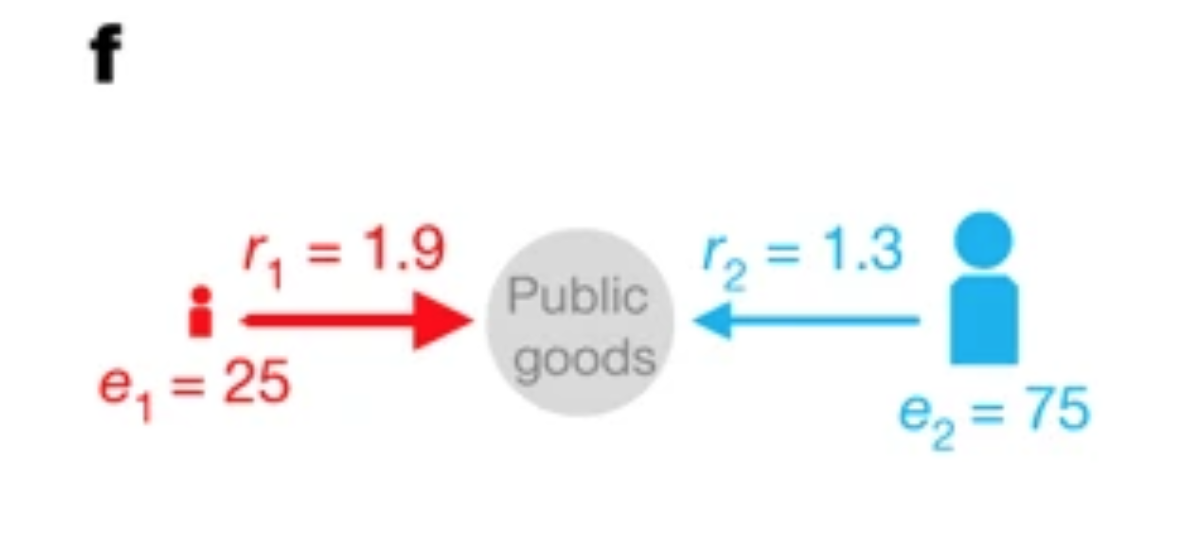
\includegraphics[width = 0.5\linewidth]{figs/2player.png}
        \caption{2 player game with subjects differ.}
    \end{figure}
\end{frame}

\begin{frame}{Realizations}
    \begin{figure}
        \centering
        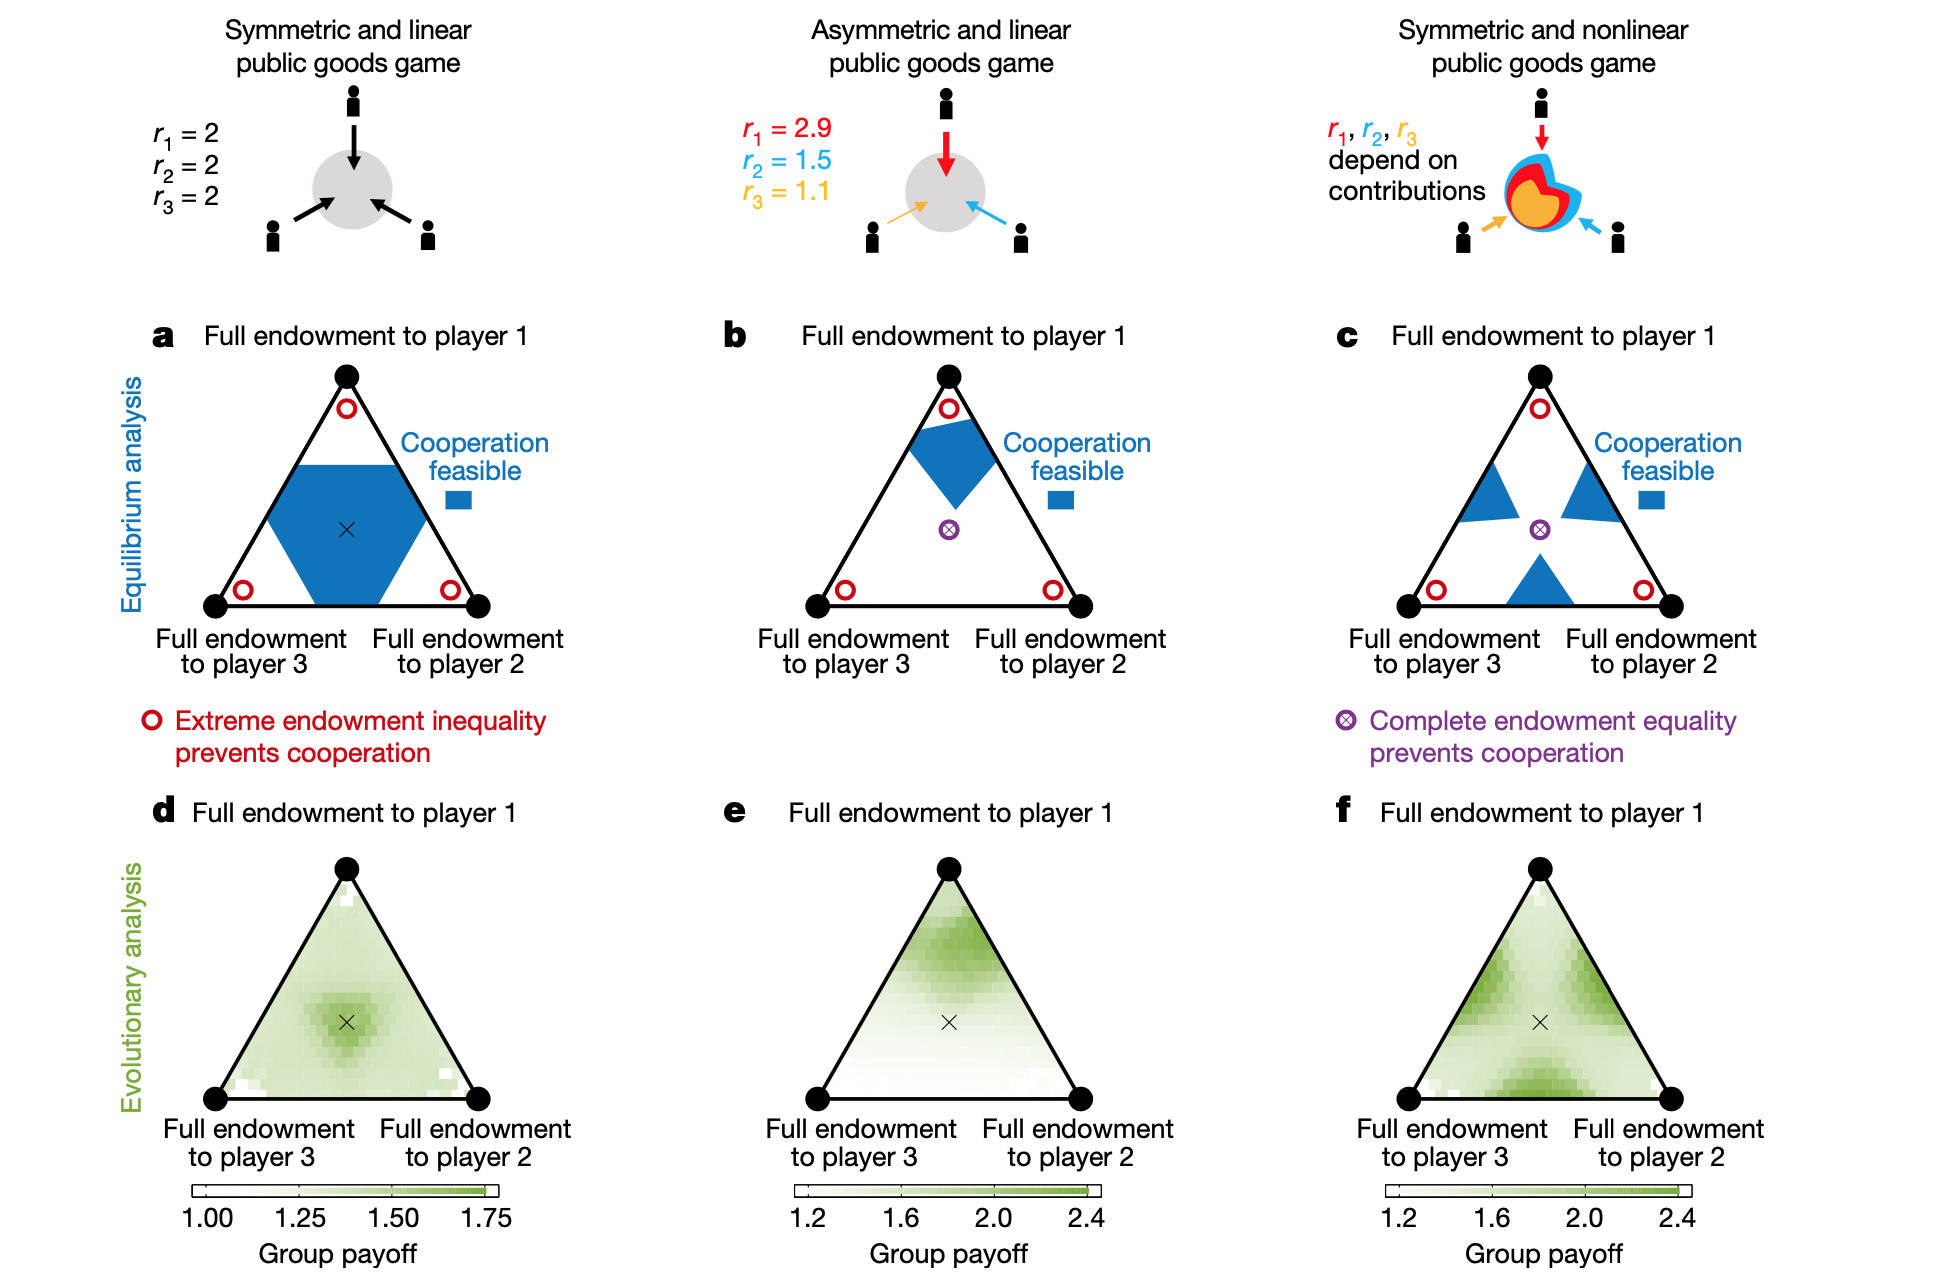
\includegraphics[width = 0.8\linewidth]{figs/realizations.png}
        \caption{When equal endowments help to maintain cooperation (a–c) or favour its evolution (d–f). }
        \label{fig:my_label}
    \end{figure}
\end{frame}

\section{合作社会如何进化}
\begin{frame}{合作社会如何演化?}
    \textbf{反馈(Respond)行为如何对未来产生影响?}

    \vspace{0.5cm}
    \textbf{一些规则}
    \begin{itemize}
        \item $x_i$只取离散值(合作-对抗)
        \item 想合作的人有$\epsilon$的概率犯错
        \item 根据payoff的变化通过随机转换规则改变策略
        
    \end{itemize}
\end{frame}
\begin{frame}{模拟演化的一些结论}
    \begin{itemize}
        \item 均质系统中,$e_i$有利于达到均衡;
        \item 不一样能干($r_i$),或者福利非线性,则不均等收益有助于达到均衡;
        \item Grim策略:因为无法容纳噪声而失效;但优胜劣汰会有利于演化出合作。
        \begin{itemize}
            \item 优胜劣汰是一个很稳定的策略。但仍会被取代。
        \end{itemize}
    \end{itemize}
\end{frame}

\begin{frame}{行为实验}
    \begin{figure}
        \centering
        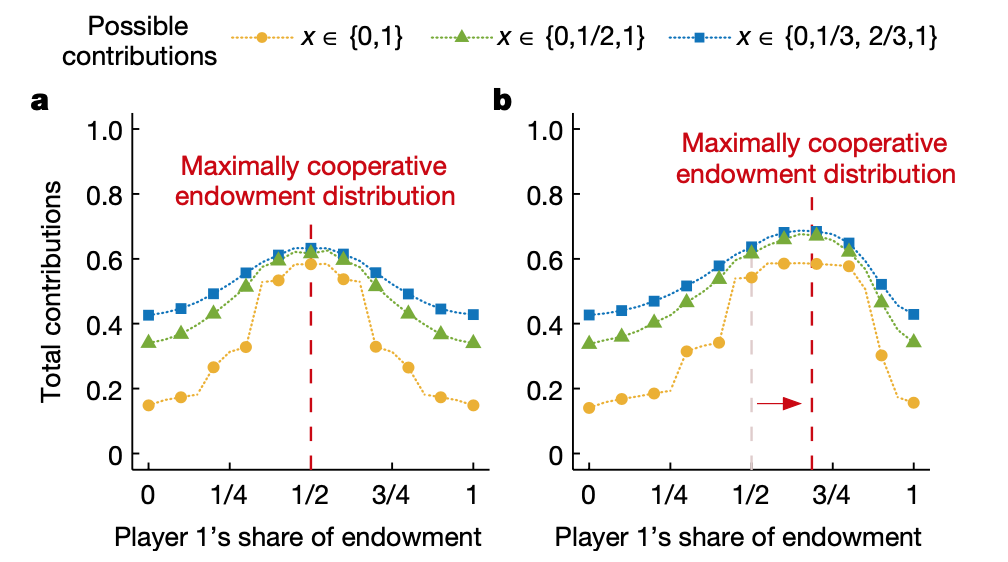
\includegraphics[width = 0.8\linewidth]{figs/Fig3.png}
        \caption{When players differ in their productivities, equal endowments do not maximize contributions. }
    \end{figure}
\end{frame}
\begin{frame}{又一个双人博弈的例子}
    环境:full equality, endowment inequality, productivity inequality, aligned inequality, misaligned inequality 
    \begin{figure}
        \centering
        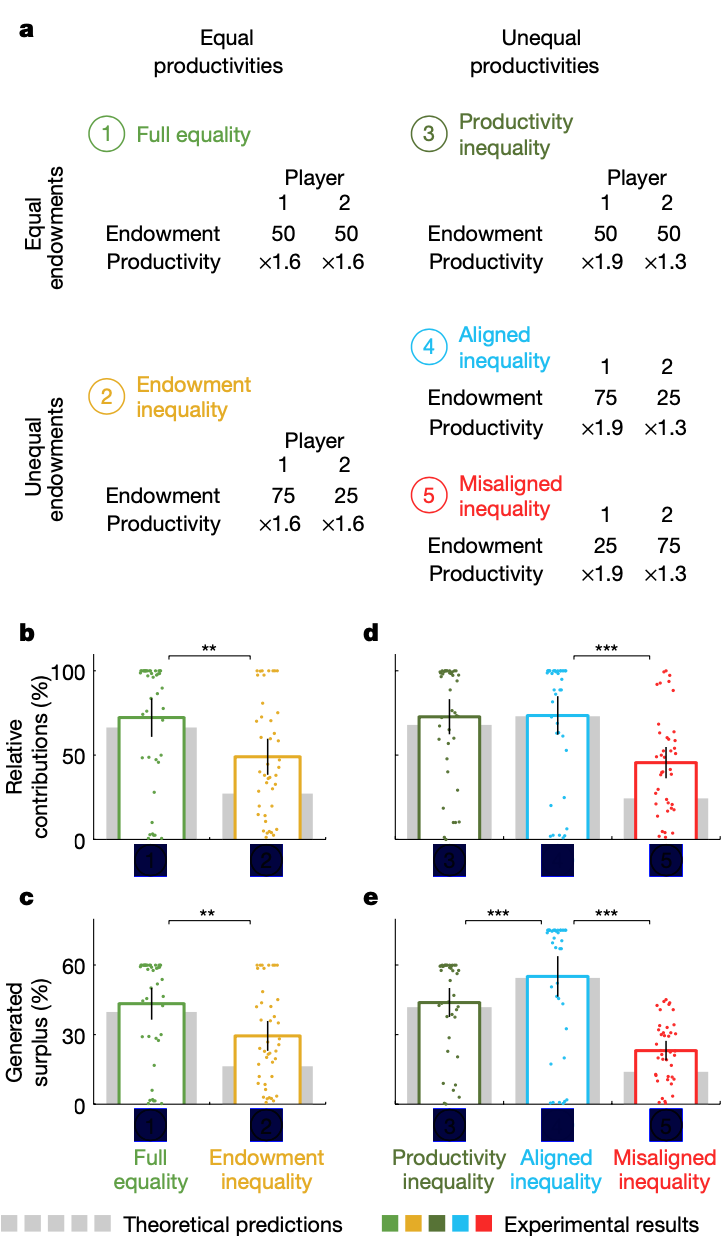
\includegraphics[width = 0.3\linewidth]{figs/Fig4.png}
        \caption{Exploring the effects of multidimensional inequality with a behavioural experiment. Players either coincide in their productivities, $r_1 =r_2 =1.6$(a), or player 1 is more productive, $r_1 =1.9$ and $r_2 =1.3$(b).}
    \end{figure}
\end{frame}

\section{总结}

\begin{frame}{总结:不平等的意义?}

\begin{itemize}
    \item 群体内部的一些不平等实际上有助于确保每个人都对群体做出足够的贡献
    \item 政策制定者确保继续支持公共产品和服务,如税收、医疗保健和教育
\end{itemize}
现象:
\begin{itemize}
    \item 非常不平等的社会中,收入较高的人不太倾向于按比例分配公共产品和服务
    \item 这也导致最低收入者贡献较少。高度不平等条件下的合作破裂对为社会提供基本服务的资金有影响。
\end{itemize}
\begin{center}
    什么情况下,不平等有害,什么情况下,不平等也会变得有益?
    
    如果不平等现象消失,公共服务将难以维持。但是太多的不平等会对每个人——既对最贫穷的人,也对富人——的后果都产生负面影响。
\end{center}
    
\end{frame}

\begin{frame}{什么是一个好的原则?}
    \begin{itemize}
        \item Bounds?
        \item Ranks?
        \item Localization?
        \item Spatial reciprocity?
        \item ......
    \end{itemize}
\end{frame}

\end{document}
